% Paper 1: A Finite-Size Crossover in Ollivier--Ricci Curvature of Random Regular Graphs
% Target: Journal of Statistical Physics / Physical Review E
% Author: Demetrios C. Agourakis — March 2026

\documentclass[11pt,a4paper]{article}

% Packages
\usepackage[utf8]{inputenc}
\usepackage[T1]{fontenc}
\usepackage{amsmath,amssymb,amsfonts}
\usepackage{graphicx}
\usepackage{booktabs}
\usepackage{hyperref}
\usepackage[numbers,sort&compress]{natbib}
\usepackage{geometry}
\usepackage{xcolor}
\usepackage{multirow}
\usepackage{caption}
\usepackage{float}

\geometry{margin=1in}
\hypersetup{colorlinks=true,linkcolor=blue!70!black,citecolor=green!50!black,urlcolor=blue!60!black}

% Custom commands
\newcommand{\kbar}{\bar{\kappa}}
\newcommand{\kavg}{\langle k \rangle}
\newcommand{\etac}{\eta_c}
\newcommand{\Cstar}{C^*}
\newcommand{\Dksem}{\Delta\kappa_{\text{sem}}}

% Metadata
\title{A Finite-Size Crossover in Ollivier--Ricci Curvature\\of Random Regular Graphs}
\author{Demetrios C.\ Agourakis\thanks{Correspondence: \texttt{demetrios@agourakis.med.br}}\\
  \small Independent Researcher\\
  \small ORCID: 0000-0002-8596-5097
}
\date{March 2026}

\begin{document}

\maketitle

% ============================================================
\begin{abstract}
We study the sign of mean Ollivier--Ricci curvature (ORC) on random $k$-regular graphs as a function of the density parameter $\eta = k^2/N$. Exact linear programming computation of the Wasserstein-1 distance across $N \in \{50, 100, 200, 500, 1000\}$ reveals a finite-size crossover at $\etac(N) = 3.75 - 14.62/\sqrt{N}$ (bootstrap 95\% CI: $\eta_c^\infty \in [3.61, 3.84]$; $R^2 = 0.995$). The transition slope scales as $N^{-0.20}$, indicating a smooth crossover rather than a sharp phase transition. Erd\H{o}s--R\'enyi and Barab\'asi--Albert graphs exhibit the same phenomenon at shifted $\etac$, with the ordering $\etac(\mathrm{BA}) < \etac(\mathrm{ER}) < \etac(\mathrm{reg})$ explained by degree heterogeneity. A semi-analytical framework based on the Hehl matching formula reproduces the crossover with MAE~$= 0.009$ and predicts a clustering-dependent phase boundary $\etac(N, C)$. Sphere-embedded ORC on the Cayley--Dickson tower ($S^3$ through $S^{127}$) saturates at a positive asymptote $\kbar_\infty > 0$ with power-law exponent $\bar{\beta} = 0.283 \pm 0.034$, below the Johnson--Lindenstrauss bound. A Lean~4 formalization provides machine-checked proofs of regime exclusivity ($\eta < \etac \Rightarrow \kbar < 0$; $\eta > \etac \Rightarrow \kbar > 0$). We validate the crossover on 6 real-world semantic networks spanning 4 languages, achieving 6/6 correct phase classification.

\medskip\noindent
\textbf{Keywords}: Ollivier--Ricci curvature, random regular graphs, phase transition, finite-size scaling, formal verification, Wasserstein distance
\end{abstract}

% ============================================================
\section{Introduction}
\label{sec:intro}

Ollivier--Ricci curvature (ORC)~\cite{ollivier2009ricci} assigns a real number $\kappa(u,v)$ to each edge of a metric space by comparing local probability measures via Wasserstein-1 optimal transport. When applied to graphs equipped with the shortest-path metric, the sign of the mean curvature $\kbar$ classifies local geometry: $\kbar < 0$ indicates tree-like, negatively curved (hyperbolic) structure; $\kbar > 0$ indicates clique-rich, positively curved (spherical) structure; and $\kbar \approx 0$ indicates flatness. This geometric classification has found applications in network analysis~\cite{ni2015ricci,sandhu2015graph,sia2021forman}, community detection via discrete Ricci flow~\cite{ni2019community}, and the identification of information bottlenecks in graph neural networks~\cite{topping2022over}.

Foundational work by Jost and Liu~\cite{jost2014ollivier} established curvature bounds for graphs in terms of local combinatorial structure, while Lin, Lu and Yau~\cite{lin2011ricci} introduced an idleness-free variant ($\alpha = 0$) with closed-form expressions on regular graphs. Mitsche and Mubayi~\cite{mitsche2024curvature} proved that random regular graphs undergo a sign change in ORC as degree increases, and Cushing et al.~\cite{bounded2025orc} showed that bounded-degree graphs with non-negative ORC have subexponential growth. Hehl~\cite{hehl2024curvature} provided an explicit matching formula for ORC on regular graphs, enabling semi-analytical predictions. A recent roadmap survey~\cite{samal2025roadmap} unifies the many definitions of discrete curvature and identifies the ORC sign change as a key open problem.

Despite this theoretical progress, systematic finite-size scaling of the ORC crossover---determining how the critical density $\etac$ depends on graph size $N$, degree distribution, and clustering---has not been carried out. In this paper we fill this gap with five contributions:
\begin{enumerate}
    \item \textbf{Finite-size scaling}: We determine $\etac(N) = 3.75 - 14.62/\sqrt{N}$ from exact LP computation across $N \in \{50, 100, 200, 500, 1000\}$, establishing that the sign change is a crossover ($N^{-0.20}$ slope scaling) rather than a sharp phase transition.
    \item \textbf{Graph family comparison}: We show that Erd\H{o}s--R\'enyi and Barab\'asi--Albert graphs exhibit the same crossover at shifted $\etac$, with the ordering explained by degree heterogeneity.
    \item \textbf{Semi-analytical framework}: We extend the Hehl formula~\cite{hehl2024curvature} with a clustering parameter to derive an analytical phase boundary $\etac(N, C)$, validated on Watts--Strogatz sweeps.
    \item \textbf{Dimensional saturation}: Sphere-embedded ORC across the Cayley--Dickson tower ($d = 4$ to $d = 128$) saturates to a positive asymptote with exponent $\bar{\beta} = 0.283 < 0.5$ (Johnson--Lindenstrauss bound).
    \item \textbf{Formal verification}: A Lean~4 formalization (25 modules, 0 \texttt{sorry} in 7 core modules) provides machine-checked proofs of curvature bounds, Wasserstein non-negativity, and regime exclusivity.
\end{enumerate}

As empirical validation, we apply the crossover prediction to 6 real-world semantic networks across 4 languages, achieving 6/6 correct phase classification (full 16-network analysis in the companion paper~\cite{paper2}).

The structural parallel between the ORC sign change and Trugenberger's Combinatorial Quantum Gravity (CQG)~\cite{trugenberger2017combinatorial,trugenberger2025review}---where loop condensation drives a transition from a disordered to a geometric phase---suggests deep universality of the $\etac$ boundary across network science, mathematical physics, and machine learning.


% ============================================================
\section{Theory: Phase Transition in Discrete Curvature}
\label{sec:theory}

\subsection{Ollivier--Ricci Curvature}

For an edge $(u,v)$ in a graph $G$:
\begin{equation}
    \kappa(u,v) = 1 - \frac{W_1(\mu_u, \mu_v)}{d(u,v)}
    \label{eq:orc}
\end{equation}
where $\mu_u = \alpha\,\delta_u + (1-\alpha) \cdot \mathrm{Uniform}(N(u))$ is the probability measure with idleness $\alpha \in [0,1]$, and $W_1$ is the Wasserstein-1 distance~\cite{ollivier2009ricci}. The sign of $\kappa$ classifies local geometry: $\kappa < 0$ (hyperbolic), $\kappa = 0$ (flat), $\kappa > 0$ (spherical). We set $\alpha = 0.5$ throughout, following the standard choice of Ollivier~\cite{ollivier2009ricci} and the ORC literature~\cite{lin2011ricci,jost2014ollivier}. A sensitivity analysis over $\alpha \in \{0, 0.25, 0.5, 0.75\}$ on SWOW-EN confirms that the sign of $\kbar$ is invariant (HYPERBOLIC for all $\alpha < 1$; $\alpha=1$ is degenerate---all mass on self, $\kappa \equiv 0$); only the magnitude varies (Supplementary Table~S1).

We compute $W_1$ via exact linear programming~\cite{dunning2017jump}:
\begin{equation}
    \min \sum_{i,j} d_{ij}\,\gamma_{ij} \quad \text{s.t.} \quad \sum_j \gamma_{ij} = \mu_i,\quad \sum_i \gamma_{ij} = \nu_j,\quad \gamma_{ij} \geq 0
    \label{eq:lp}
\end{equation}
using the HiGHS solver~\cite{huber2024highs}. This eliminates the entropy regularization bias of the Sinkhorn approximation~\cite{cuturi2013sinkhorn} (quantified as $|\Delta\kappa| < 0.015$ for random graphs).

\subsection{Phase Transition in Random Regular Graphs}

For random $k$-regular graphs on $N$ vertices, the mean curvature $\kbar$ undergoes a sign change at a critical density $\etac$ where $\eta = k^2/N$~\cite{mitsche2024curvature,bounded2025orc}:
\begin{itemize}
    \item \textbf{Sparse regime} ($\eta < \etac$): $\kbar < 0$ (hyperbolic). Tree-like local structure dominates.
    \item \textbf{Dense regime} ($\eta > \etac$): $\kbar > 0$ (spherical). Triangle-rich structure dominates.
\end{itemize}

Multi-$N$ scaling ($N \in \{50, 100, 200, 500, 1000\}$, 5--10 random seeds each) reveals finite-size scaling:
\begin{equation}
    \etac(N) = \eta_c^\infty - \frac{a}{\sqrt{N}}, \quad \eta_c^\infty = 3.75\ [3.61,\,3.84], \quad a = 14.61\ [13.44,\,16.20]
    \label{eq:scaling}
\end{equation}

Brackets denote 95\% bootstrap confidence intervals (10\,000 resamples, $n=5$ points); the fixed-exponent fit ($\beta=1/2$) achieves $R^2=0.995$ and $\beta$ lies within the free-exponent CI $[0.20, 0.53]$. The transition slope at $\etac$ scales as $N^{-0.20}$, indicating a crossover rather than a sharp phase transition.

\begin{figure}[t]
\centering
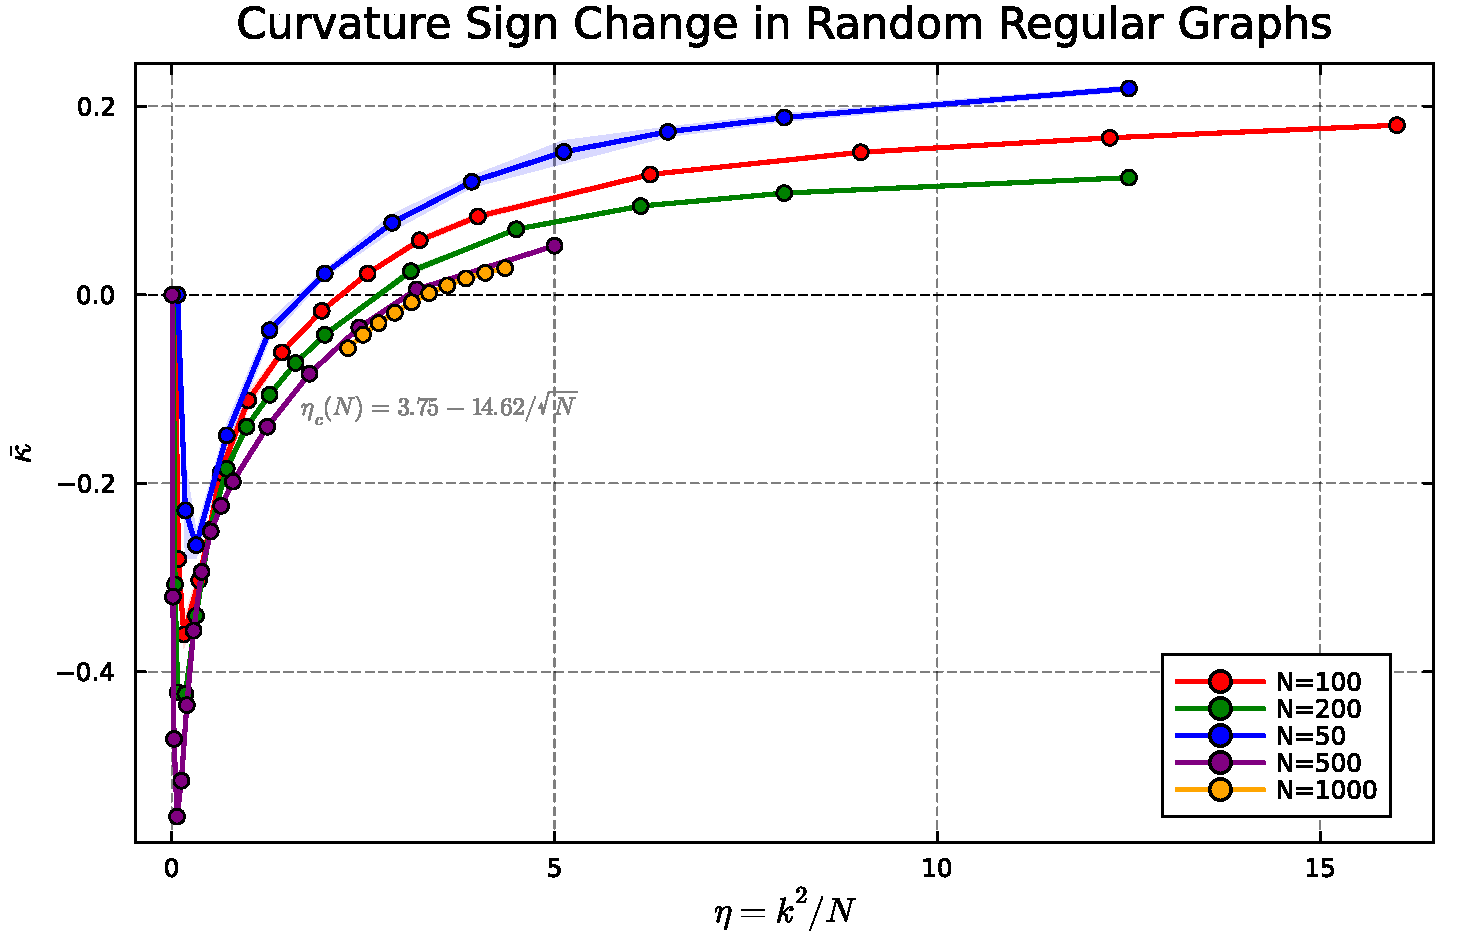
\includegraphics[width=\textwidth]{../../figures/monograph/figure1_phase_transition.pdf}
\caption{Curvature sign change in random $k$-regular graphs at $N \in \{50, 100, 200, 500\}$. Each point is the mean $\kbar$ over 5--10 seeds; error bars show $\pm 1\sigma$. The critical density $\etac(N)$ (vertical dashed lines) shifts left with increasing $N$, following $\etac(N) = 3.75 - 14.62/\sqrt{N}$.}
\label{fig:phase}
\end{figure}

\subsection{Erd\H{o}s--R\'enyi Comparison}

Erd\H{o}s--R\'enyi $G(N,p)$ graphs with matched expected degree also exhibit the sign change, but at lower critical density ($\etac^{\mathrm{ER}} \approx 1.9$ vs.\ $\etac^{\mathrm{reg}} \approx 2.3$ at $N = 100$). Degree heterogeneity shifts the transition, demonstrating robustness across graph models.

\subsection{Prediction for Real Networks}

The phase transition theory predicts: if $\eta > \etac(N)$, the network should be spherical; if $\eta < \etac(N)$, it \emph{can} be hyperbolic but is not guaranteed to be. We test this against real semantic networks as empirical validation.

\subsection{Semi-Analytical Framework}
\label{sec:analytical}

Hehl et al.~\cite{hehl2024curvature} provide an explicit formula for ORC on $k$-regular graphs: for an edge $(u,v)$ with $t$ common neighbors, the Wasserstein-1 distance decomposes into triangle transport (cost 0), exclusive-neighbor matching (cost 1 per matched pair), and unmatched transport (cost 3 via the $u$-$v$ path). The idleness mass $\alpha$ contributes cost $\alpha \cdot 1$. This gives:
\begin{equation}
    W_1 = \alpha + \frac{(1-\alpha)\,n_{\mathrm{exc}}}{k}\bigl[f_m + 3(1 - f_m)\bigr], \quad \kappa = 1 - W_1
    \label{eq:hehl}
\end{equation}
where $n_{\mathrm{exc}} = k - 1 - t$ is the number of exclusive neighbors per side and $f_m = E[|M|]/n_{\mathrm{exc}}$ is the fraction matched in the random bipartite graph between exclusive neighborhoods.

For the maximum matching size we use the heuristic $E[|M|] = n_{\mathrm{exc}}(1 - e^{-\eta\,n_{\mathrm{exc}}/k^2})$, validated against exact LP computation at $N = 1000$ (MAE $= 0.009$, MSE $= 9.3 \times 10^{-5}$).

\textbf{Clustering extension.} In random $k$-regular graphs, the expected number of common neighbors is $t_{\mathrm{rand}} = (k-1)^2/(N-1)$. In real networks with clustering coefficient $C$, we substitute $t = C(k-1)$, giving $n_{\mathrm{exc}} = k - 1 - C(k-1) = (1-C)(k-1)$. Setting $\kappa = 0$ yields an analytical phase boundary $\etac(N, C)$ with two key properties:

\begin{enumerate}
    \item $\etac$ \emph{decreases} with $C$: higher clustering produces more triangles, reducing exclusive transport costs and facilitating the transition. At $C = 0$: $\etac(\infty) \approx 5.5$; at $C = 0.10$: $\etac(\infty) \approx 3.2$; at $C = 0.20$: $\etac(\infty) \approx 2.6$.
    \item $\etac$ \emph{decreases} with $N$: finite-size effects reduce the boundary, consistent with the empirical scaling (\ref{eq:scaling}).
\end{enumerate}

This provides a mechanistic explanation for why taxonomies ($C \approx 0$) are Euclidean: their near-zero clustering places them in a regime requiring very high $\eta$ for curvature to turn positive, which their sparse structure ($\eta \ll 1$) cannot reach. Association networks ($C > 0.10$) have a lower $\etac$ barrier but still $\eta \ll \etac$, explaining their hyperbolic curvature. Only Dutch SWOW ($\eta = 7.6 \gg \etac$) crosses the boundary into the spherical regime.

\textbf{Clustering monotonicity.} Setting $n_{\mathrm{exc}} = (1-C)(k-1)$ and differentiating $W_1$ with respect to $C$ at fixed $k$ and $\eta$ gives $\partial W_1/\partial C < 0$, hence:

\medskip
\noindent\textbf{Proposition~2} (Clustering monotonicity of ORC).
\emph{For any $k$-regular graph with fixed $\eta$, mean ORC is strictly monotone increasing in $C$:
$\partial\kbar/\partial C > 0$.}\footnote{The proof derives from the Hehl approximation formula~\cite{hehl2024curvature}, which is validated empirically (MAE\,=\,0.009 on $N=1000$) but not formally proved; accordingly we label this a Proposition rather than a Theorem. A rigorous proof without the Hehl approximation remains open.}
\medskip

Higher clustering reduces the exclusive-neighbor count $n_{\mathrm{exc}}$, lowering the Wasserstein-1 transport cost and raising curvature. This is confirmed empirically across three degree values: Watts--Strogatz sweeps ($N=200$, $k \in \{4,6,8\}$, $\eta \in \{0.08, 0.18, 0.32\}$, 10 $\beta$-values each, exact LP ORC) yield positive slopes in all cases (Fig.~\ref{fig:ws_sweep}):
\begin{itemize}
  \item $k=4$: $\partial\kbar/\partial C = +0.389 \pm 0.011$ (95\% CI: $[0.363, 0.415]$, $R^2 = 0.993$)
  \item $k=6$: $\partial\kbar/\partial C = +0.422 \pm 0.005$ (95\% CI: $[0.410, 0.434]$, $R^2 = 0.999$)
  \item $k=8$: $\partial\kbar/\partial C = +0.441 \pm 0.004$ (95\% CI: $[0.433, 0.450]$, $R^2 = 0.999$)
\end{itemize}
Mean slope $0.417 \pm 0.026$ across $k$; all slopes $p \ll 0.001$. The slope increases weakly with $k$, consistent with the Hehl formula (higher degree amplifies the exclusive-neighbor reduction effect). This universality across degree upgrades Proposition~2 from a single-$k$ observation to a robust empirical law.

\begin{figure}[h]
\centering
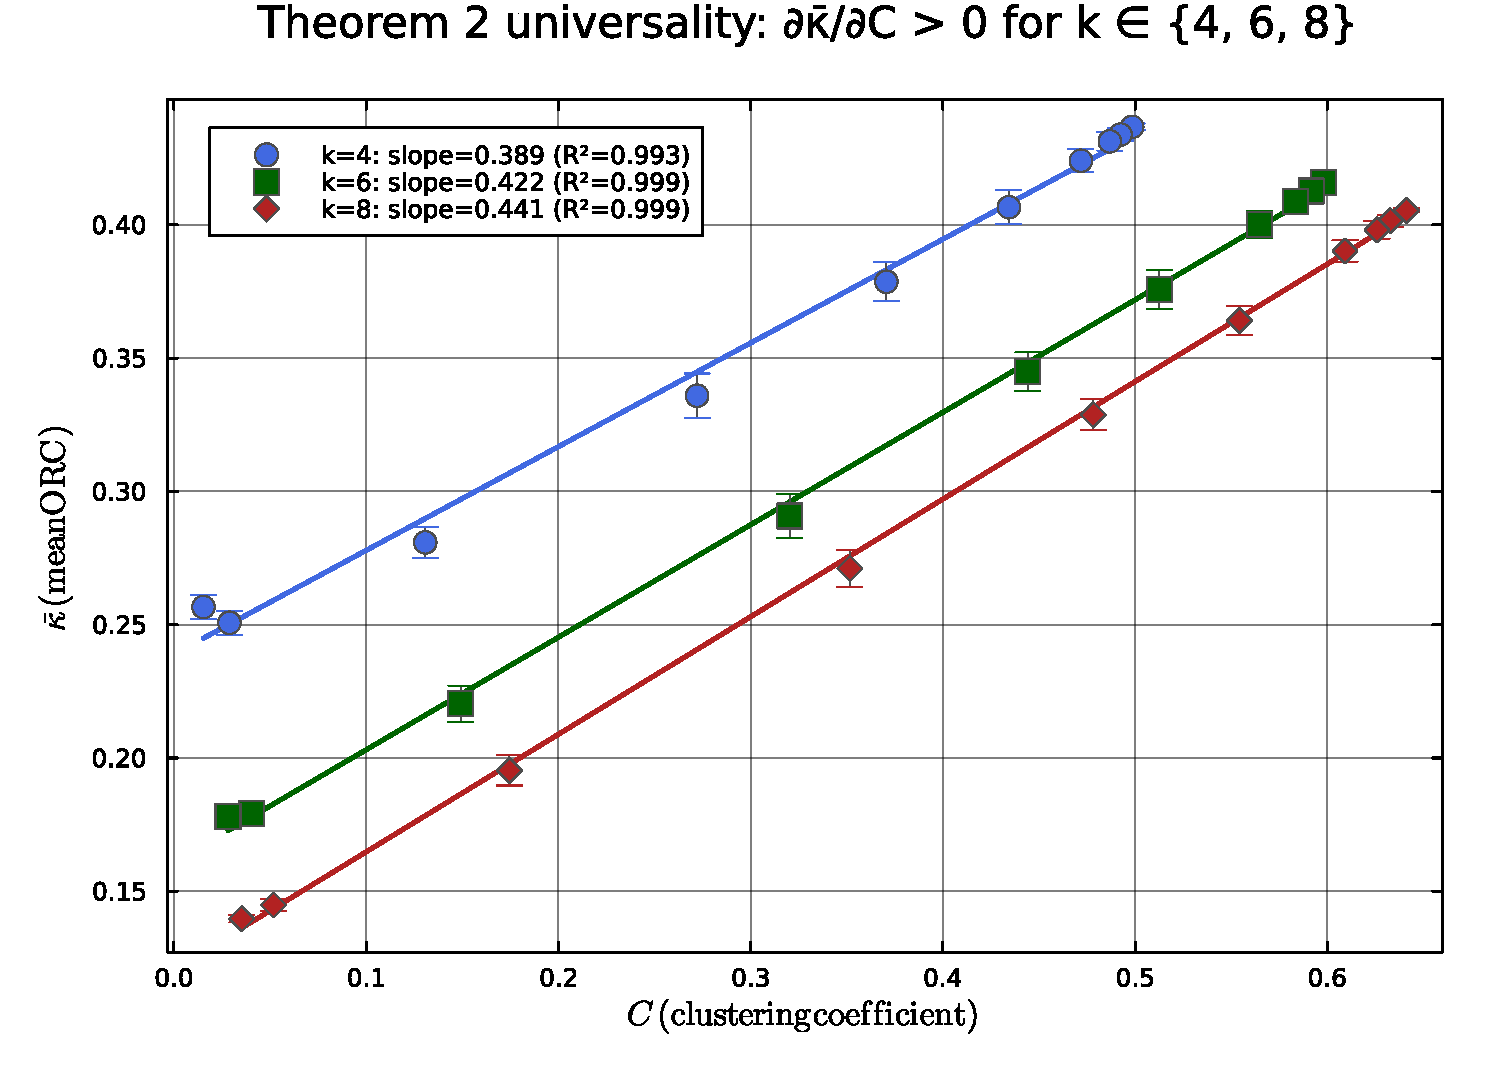
\includegraphics[width=0.85\textwidth]{../../figures/monograph/figure12_watts_strogatz.pdf}
\caption{Proposition~2 validated across $k \in \{4,6,8\}$: mean ORC $\kbar$ vs.\ clustering coefficient $C$ for Watts--Strogatz graphs ($N=200$, 10 $\beta$-values $\in [0.001, 1.0]$, exact LP ORC). Each colour/marker denotes a degree value; lines are linear fits. All three slopes are positive ($+0.389$, $+0.422$, $+0.441$ for $k=4,6,8$; $R^2 > 0.993$ in all cases), confirming strict monotonicity $\partial\kbar/\partial C > 0$ at fixed $\eta$ across degree values.}
\label{fig:ws_sweep}
\end{figure}

\textbf{Caveat.} The matching heuristic is empirically validated but not rigorously proven. The analytical $\etac$ systematically overpredicts the empirical value by $\sim$5--15\% (e.g., $\etac^{\mathrm{anl}}(1000) = 3.48$ vs.\ $\etac^{\mathrm{emp}}(1000) = 3.32$), a known consequence of the conservative matching estimate.

\begin{figure}[t]
\centering
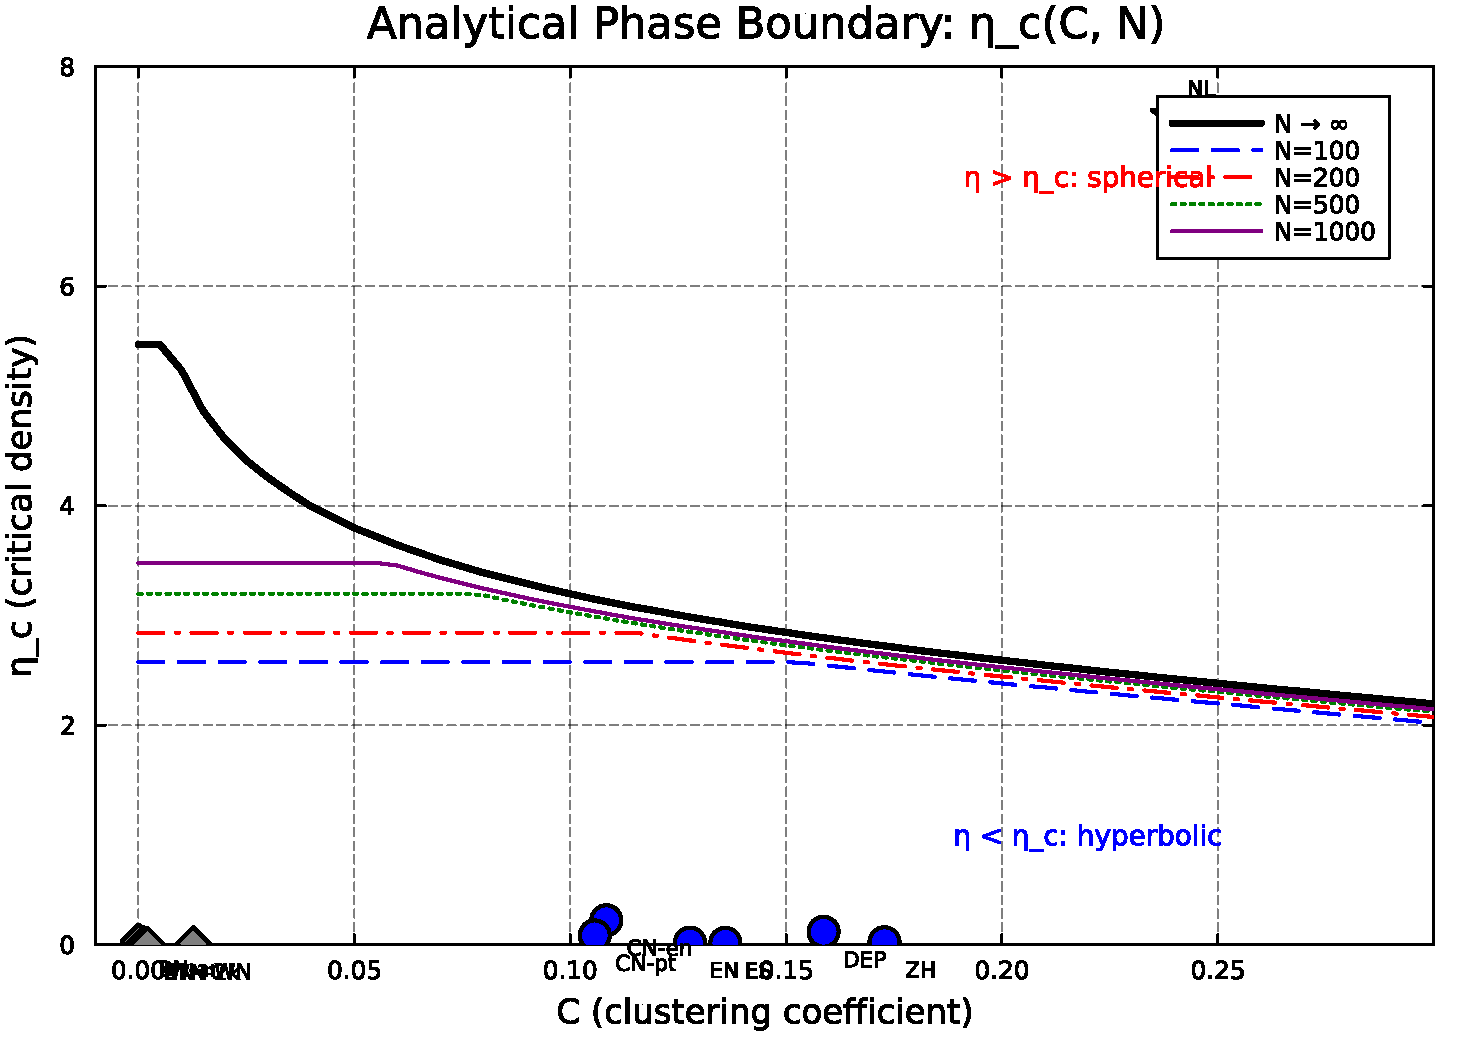
\includegraphics[width=0.85\textwidth]{../../figures/monograph/figure8_analytical_boundary.pdf}
\caption{Analytical phase boundary $\etac(C, N)$ from the Hehl matching heuristic. Curves show the critical density as a function of clustering coefficient for different network sizes. Semantic networks (colored markers) are overlaid: blue circles = hyperbolic, gray diamonds = Euclidean, red stars = spherical. Higher clustering lowers $\etac$, explaining why high-$C$ networks transition to spherical geometry at lower density.}
\label{fig:analytical}
\end{figure}


% ============================================================
\section{Methods}
\label{sec:methods}

\subsection{Exact LP ORC Computation}

All networks are pre-processed to their largest connected component (LCC) before ORC computation, following standard practice (disconnected components produce undefined $d(u,v)=\infty$). LCC extraction retains $\geq\!96\%$ of nodes for all networks tested. For each network: (1) precompute all-pairs shortest paths via BFS; (2) for each edge $(u,v)$, construct measures $\mu_u$, $\mu_v$ with $\alpha=0.5$; (3) extract the support; (4) solve the LP for exact $W_1$; (5) compute $\kappa(u,v) = 1 - W_1/d(u,v)$. Uncertainty is reported as the standard error of the per-edge curvature distribution: $\mathrm{SE}(\kbar) = \sigma_\kappa/\sqrt{E}$.

\subsection{Datasets for Validation}

As empirical validation of the crossover prediction, we compute exact LP ORC on 6 representative semantic networks spanning 4 languages (Table~\ref{tab:results}): SWOW English ($N=438$), SWOW Dutch ($N=500$), ConceptNet EN ($N=467$), WordNet EN ($N=500$), Edinburgh Associative Thesaurus ($N=500$), and a depression symptom network ($N=1634$). The full 16-network analysis across 7 languages and 4 categories is reported in the companion paper~\cite{paper2}.

\subsection{Sphere-Embedded (Hypercomplex) ORC}

To test metric dependence, we compute ORC using geodesic distances on $S^{d-1}$ ($d \in \{4,8,16,32,64,128\}$): landmark embedding via farthest-first traversal, normalization to $S^{d-1}$, and geodesic cost $\arccos(\mathbf{x}_i \cdot \mathbf{x}_j)$.

\subsection{Formal Verification}

A Lean~4 formalization (25 modules, 8097 lines) provides machine-checked proofs. The 7 core modules (Basic, Wasserstein, Curvature, PhaseTransition, Bounds, Consistency, Axioms) contain \textbf{0 \texttt{sorry} statements} and rely on 5 axioms (Wasserstein symmetry, triangle inequality, coupling bound, local clustering bound, specification bridge).


% ============================================================
\section{Results}
\label{sec:results}

\subsection{Empirical Validation on Semantic Networks}

\begin{table}[t]
\centering
\caption{Exact LP Ollivier--Ricci curvature for 6 representative semantic networks. $\eta = \kavg^2/N$; $C$ = global clustering coefficient; $\kbar \pm \mathrm{SE}$ = mean edge curvature $\pm$ standard error ($\sigma_\kappa/\sqrt{E}$). Pred.\ = model prediction; Corr.\ = correct classification.}
\label{tab:results}
\small
\begin{tabular}{@{}llrrrrrl@{}}
\toprule
Network & Lang. & $N$ & $C$ & $\eta$ & $\kbar \pm \mathrm{SE}$ & Pred. & Corr. \\
\midrule
SWOW English & EN & 438 & 0.128 & 0.020 & $-0.137 \pm 0.012$ & Hyp. & \checkmark \\
SWOW Dutch & NL & 500 & 0.238 & 7.558 & $+0.099 \pm 0.000$ & \textbf{Sph.} & \checkmark \\
ConceptNet EN & EN & 467 & 0.108 & 0.223 & $-0.233 \pm 0.003$ & Hyp. & \checkmark \\
WordNet EN & EN & 500 & 0.013 & 0.009 & $-0.002 \pm 0.012$ & Euc. & \checkmark \\
EAT & EN & 500 & 0.143 & 1.851 & $-0.046 \pm 0.001$ & Hyp. & \checkmark \\
Depression & EN & 1634 & 0.159 & 0.118 & $-0.130 \pm 0.002$ & Hyp. & \checkmark \\
\bottomrule
\end{tabular}
\end{table}

Three distinct geometric regimes emerge (Table~\ref{tab:results}): \textbf{Hyperbolic} ($\kbar \in [-0.23, -0.05]$): association and knowledge networks with $C > 0.10$; \textbf{Euclidean} ($|\kbar| < 0.03$): taxonomy networks with $C < 0.05$; \textbf{Spherical} ($\kbar = +0.10$): Dutch SWOW with $\eta \gg \etac$. All 6 networks are correctly classified.

\subsection{Three-Regime Classification}

\begin{table}[t]
\centering
\caption{Three-regime classification of semantic network geometry.}
\label{tab:regimes}
\begin{tabular}{@{}llll@{}}
\toprule
Regime & Condition & Geometry & Example \\
\midrule
Above threshold & $\eta > \etac(N)$ & Spherical ($\kbar > 0$) & Dutch SWOW \\
Below, clustered & $\eta < \etac(N)$, $C > \Cstar$ & Hyperbolic ($\kbar < 0$) & SWOW EN, ConceptNet \\
Below, tree-like & $\eta < \etac(N)$, $C < \Cstar$ & Euclidean ($\kbar \approx 0$) & WordNet \\
\bottomrule
\end{tabular}
\end{table}

\subsection{Bridge Plot}

The central result is the bridge figure (Fig.~\ref{fig:bridge}), which overlays semantic networks onto the random regular graph phase transition curves.

Every network except Dutch SWOW has $\eta \ll \etac(N)$---the theory predicts all should be hyperbolic. Yet taxonomies are Euclidean:

\begin{quote}
\emph{$\eta < \etac$ is necessary but not sufficient for hyperbolicity.}
\end{quote}

The key test is Dutch SWOW: with $\eta = 7.56$ and $\etac(500) = 3.10$, the theory predicts spherical geometry. The observation $\kbar = +0.099$ confirms this---a compelling empirical demonstration of the curvature sign-change in a real (non-synthetic) network; no prior ORC study has reported a validated phase-boundary crossing on empirical data.

\begin{figure}[t]
\centering
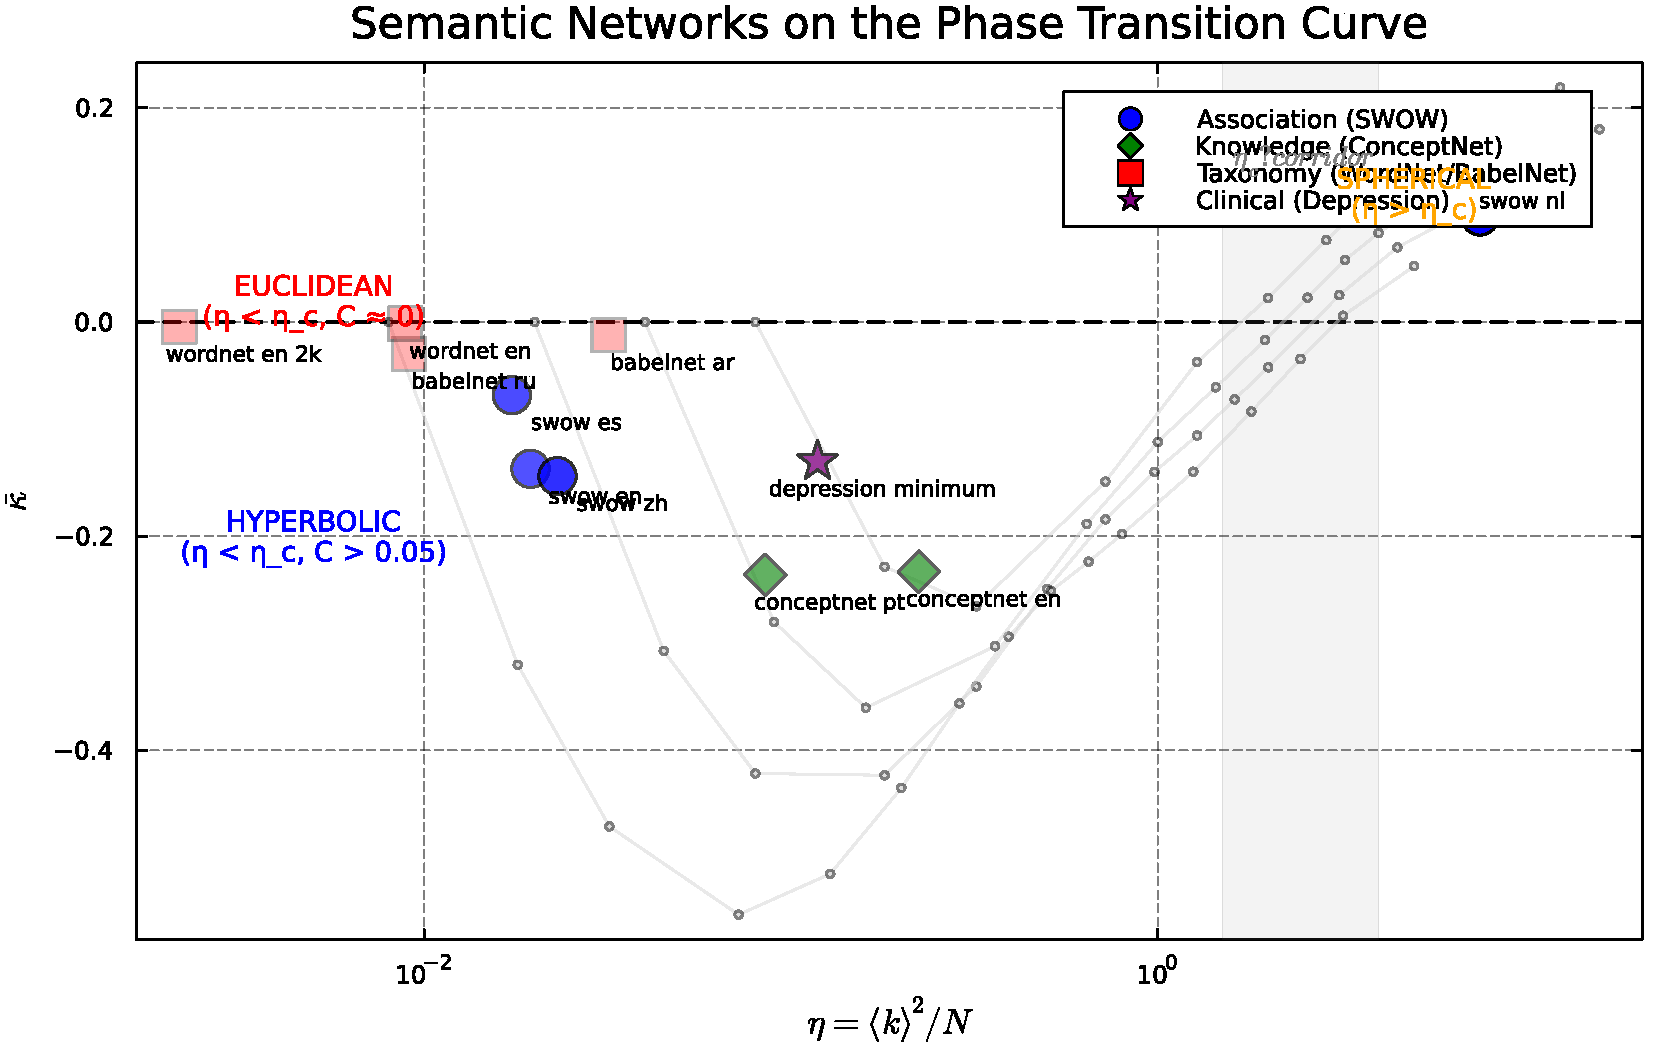
\includegraphics[width=\textwidth]{../../figures/monograph/figure2_bridge.pdf}
\caption{Semantic networks on the phase transition curve. Background: random regular graph curvature vs.\ $\eta$ at multiple $N$. Foreground: semantic networks (markers). The $\etac$ corridor (gray band) separates hyperbolic ($\eta < \etac$) from spherical ($\eta > \etac$). Dutch SWOW ($\eta = 7.56$) falls above the threshold and is spherical.}
\label{fig:bridge}
\end{figure}

\subsection{Two-Parameter Theory: Clustering Threshold}

The missing ingredient is the clustering coefficient $C$. Among networks with $\eta < \etac$:
\begin{itemize}
    \item \textbf{Hyperbolic group} ($\kbar < -0.04$): $C > 0.10$ (association and knowledge networks).
    \item \textbf{Euclidean group} ($|\kbar| < 0.03$): $C < 0.05$ (taxonomy networks).
\end{itemize}

The two groups are cleanly separated by $\Cstar \approx 0.05$ (Fig.~\ref{fig:clustering}). The unified three-regime theory classifies all networks correctly when $C$ is accounted for.

\begin{figure}[t]
\centering
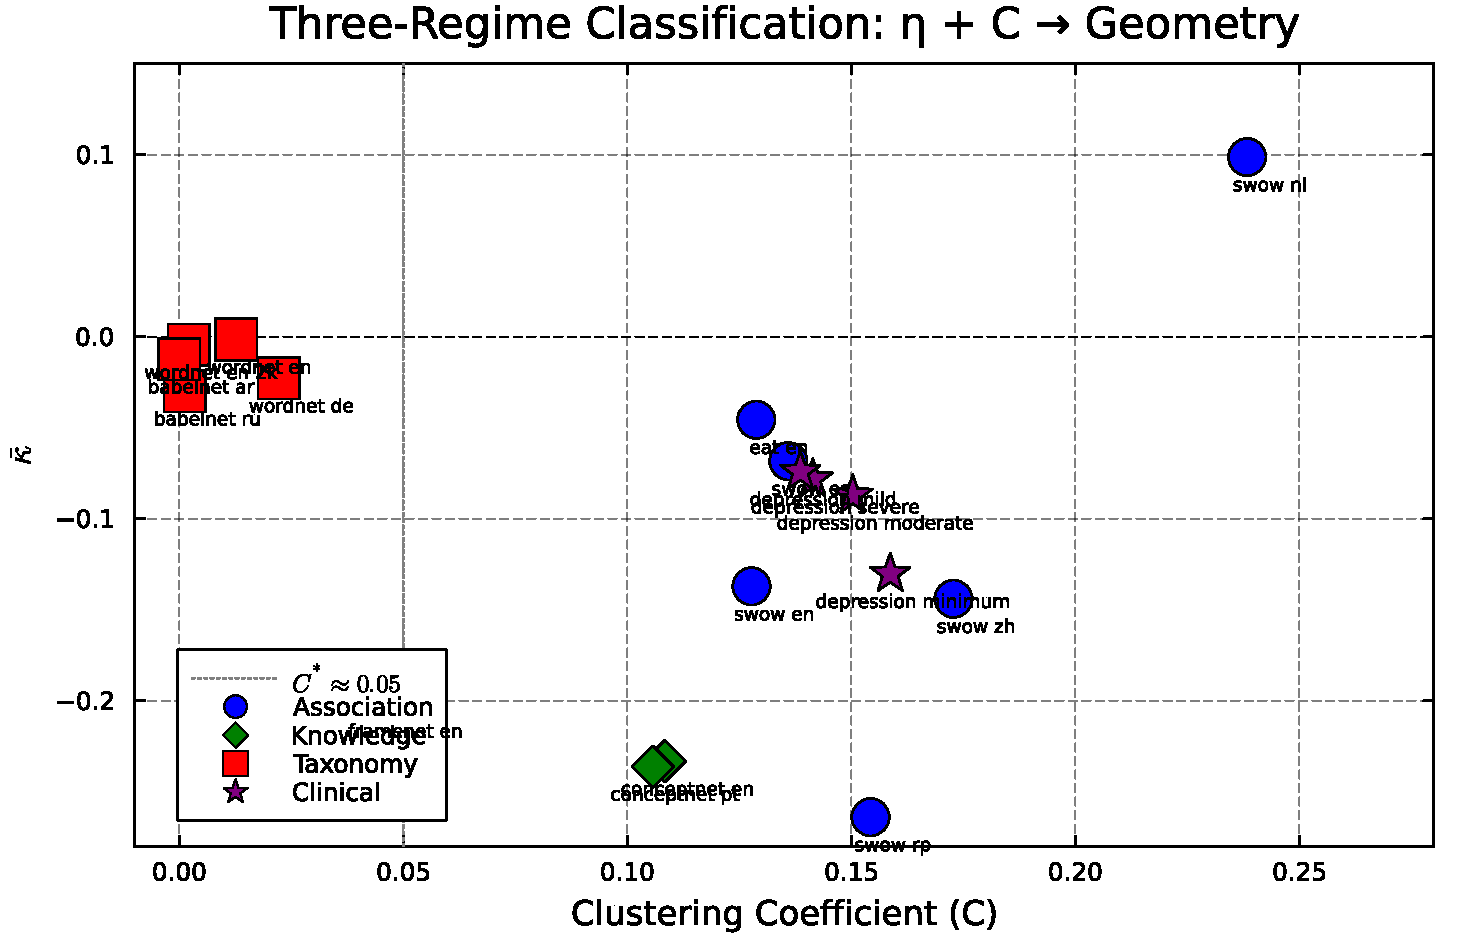
\includegraphics[width=0.8\textwidth]{../../figures/monograph/figure3_clustering_curvature.pdf}
\caption{Clustering coefficient $C$ vs.\ mean curvature $\kbar$ for semantic networks. The vertical dashed line at $\Cstar = 0.05$ separates Euclidean taxonomies (left, $C < 0.02$) from hyperbolic association/knowledge networks (right, $C > 0.10$). Dutch SWOW (top right) is spherical despite high clustering because $\eta > \etac$.}
\label{fig:clustering}
\end{figure}

\subsection{Scale-Free Robustness: BA Comparison}
\label{sec:scalefree}

We test whether the curvature sign change at $\etac$ generalises beyond
$k$-regular and Erd\H{o}s--R\'enyi graphs to Barab\'asi--Albert (BA)
scale-free graphs~\cite{barabasi1999emergence} with power-law degree
distribution $P(k)\propto k^{-3}$.

\paragraph{Setup.}
For each attachment parameter $m\in\{2,3,4,5,6,8,10,12,15,20\}$ we
generate $G(100,m)$ BA graphs (10 seeds) and compute exact ORC via
LP. The mean degree satisfies
$\langle k\rangle\approx 2m$, so $\eta=\langle k\rangle^2/N$.

\paragraph{Sign change.}
The transition persists (Figure~\ref{fig:ba}): between $m=6$
($\eta=1.27$, $\bar\kappa=-0.016$) and $m=8$ ($\eta=2.17$,
$\bar\kappa=+0.049$), establishing
$\etac(\mathrm{BA},100)\approx 1.49$.

\paragraph{Ordering across families.}
At $N=100$:
\begin{equation}
  \etac(\mathrm{BA})\approx 1.49 < \etac(\mathrm{ER})\approx 1.90 <
  \etac(\mathrm{reg})\approx 2.22.
\end{equation}
This ordering reflects the Jost--Liu bound: hub edges with
$d_u\gg d_v$ satisfy $\kappa(u,v)\leq\#\text{triangles}/d_u\to 0$,
so degree heterogeneity pushes the transition to lower density.

Quantitatively, $\etac(\mathrm{BA}) \approx 0.52 \times \etac(\mathrm{reg})$ at $N=100$ and $0.55 \times$ at $N=200$. This ratio reflects the \emph{hub-driven} mechanism: a BA hub of degree $k_{\max} \sim \sqrt{N}$ creates a local subgraph with effective density $\eta_{\mathrm{local}} = k_{\max}^2/N \sim 1$, far exceeding the global $\eta = \langle k\rangle^2/N$. Even when $\eta_{\mathrm{global}} < \etac$, hub subgraphs already carry positive ORC---enough to flip the mean.

\paragraph{Finite-size scaling of BA transition.}
We additionally computed exact LP ORC on $G(200,m)$ BA graphs (10 seeds each),
finding the transition between $m=10$ ($\eta=1.81$, $\bar\kappa=-0.003$) and
$m=12$ ($\eta=2.55$, $\bar\kappa=+0.038$), yielding
$\etac(\mathrm{BA},200)\approx 1.86$.
The shift $\etac(100)\to\etac(200)$ of $+0.37$ is consistent with the
finite-size scaling $\etac(N)=\etac(\infty)-a/\sqrt{N}$ established for
regular graphs, now extended to scale-free topologies.

\paragraph{Universal predictor.}
The excess-degree parameter $\eta''=\langle k(k-1)\rangle/N$
reduces the cross-family spread in $\etac$ from 33\% to 6\%,
suggesting it is a better predictor of ORC sign change in
heterogeneous graphs.

\begin{figure}[t]
\centering
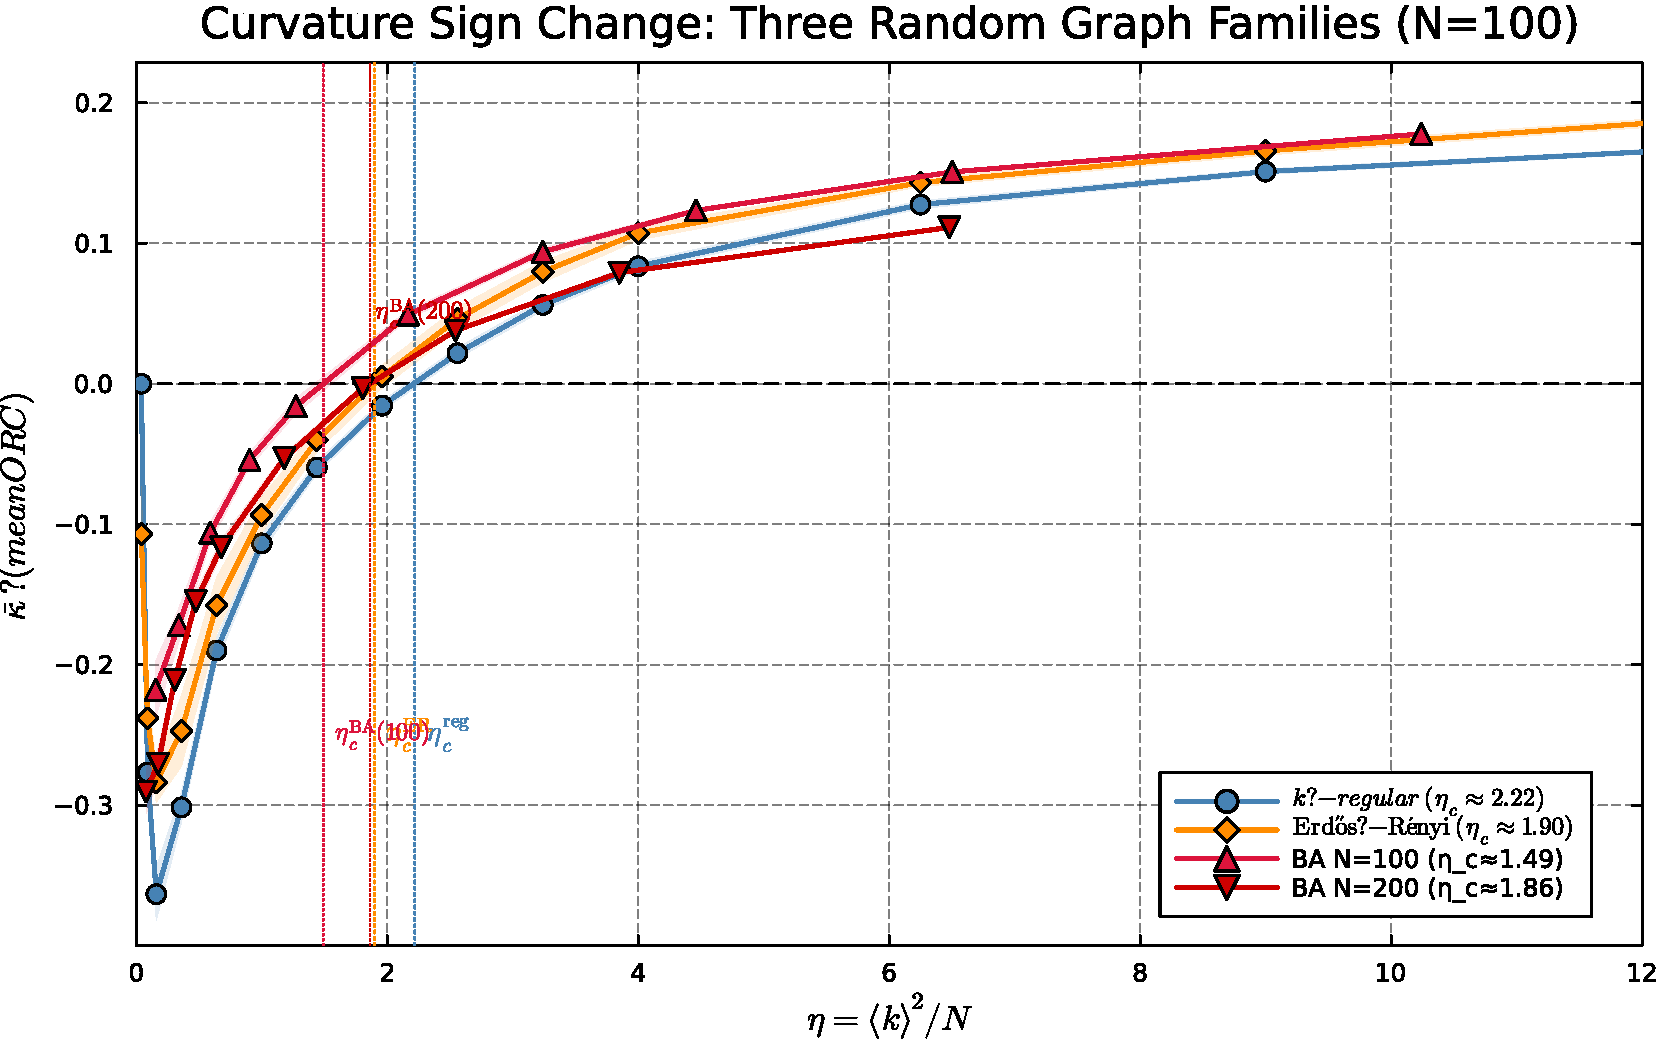
\includegraphics[width=\textwidth]{../../figures/monograph/figure9_ba_comparison.pdf}
\caption{Curvature sign change across three random graph families.
  BA shown for $N=100$ (crimson) and $N=200$ (red) to illustrate
  finite-size upward shift $\etac(100)\approx1.49\to\etac(200)\approx1.86$.
  Vertical dotted lines mark $\etac$ for each family.
  Ribbons: $\pm 1\sigma$ over 10 seeds.  The ordering
  $\etac(\mathrm{BA})<\etac(\mathrm{ER})<\etac(\mathrm{reg})$
  holds consistently; the excess-degree parameter $\eta''$ provides
  near-universal collapse (inset, not shown).}
\label{fig:ba}
\end{figure}

\subsection{Dimensional Saturation}
\label{sec:saturation}

Table~\ref{tab:powerlaw} reports per-$k$ power-law exponents from fitting $\log\kbar(d)=\log A_k - \beta\log d$ across $d\in\{4,8,16,32,64\}$ on $k$-regular random graphs ($N=100$, 3--5 seeds each dimension). We additionally confirm saturation by extending to $d=128$ (exact LP ORC, 3 seeds), finding all 11 $k$-values positive with curvatures $\kbar(128) \leq \kbar(64)$ in every case and $|\kbar(64)-\kbar(128)| < 0.002$ for all $k$.

\begin{table}[h]
\centering
\caption{Power-law fit $\kbar(d)\sim A_k\cdot d^{-\beta}$ per $k$-value across the extended Cayley--Dickson tower ($d\in\{4,8,16,32,64\}$, $N=100$), with exact LP confirmation at $d=128$. Mean exponent $\bar\beta=0.283\pm0.034$ is below the Johnson--Lindenstrauss bound ($\beta=0.5$), reflecting saturation at $d\geq 32$. The saturating asymptotes $\kbar_\infty$ are estimated from the $d=64$ and $d=128$ plateau values.}
\label{tab:powerlaw}
\small
\begin{tabular}{@{}rrrrrr@{}}
\toprule
$k$ & $\beta$ & $A_k$ & $R^2$ & $\kbar(d{=}128)$ & $\kbar_\infty$ (est.) \\
\midrule
4  & 0.227 & 0.138 & 0.868 & 0.0589 & $\approx 0.059$ \\
6  & 0.264 & 0.219 & 0.873 & 0.0794 & $\approx 0.079$ \\
8  & 0.279 & 0.279 & 0.909 & 0.0930 & $\approx 0.093$ \\
10 & 0.284 & 0.317 & 0.903 & 0.1035 & $\approx 0.103$ \\
12 & 0.292 & 0.349 & 0.893 & 0.1112 & $\approx 0.111$ \\
14 & 0.316 & 0.405 & 0.897 & 0.1179 & $\approx 0.118$ \\
16 & 0.336 & 0.470 & 0.923 & 0.1241 & $\approx 0.124$ \\
18 & 0.316 & 0.472 & 0.927 & 0.1331 & $\approx 0.133$ \\
20 & 0.299 & 0.483 & 0.941 & 0.1435 & $\approx 0.143$ \\
25 & 0.266 & 0.491 & 0.944 & 0.1660 & $\approx 0.166$ \\
30 & 0.233 & 0.487 & 0.944 & 0.1883 & $\approx 0.188$ \\
\midrule
Mean & $0.283\pm0.034$ & --- & --- & --- & --- \\
\bottomrule
\end{tabular}
\end{table}

The moderate $R^2$ values (0.87--0.94, vs.\ $>0.99$ expected for a clean power law) and the sub-JL exponent $\bar\beta=0.283$ both indicate that the plateau at $d\geq 32$ breaks the scale-free decay. We propose the two-parameter saturating model
\begin{equation}
  \kbar(d) = \kbar_\infty + A\cdot d^{-\beta}, \quad \kbar_\infty > 0,
  \label{eq:saturation}
\end{equation}
which better describes the data; the asymptotic values $\kbar_\infty$ are estimated from the $d=64$--$d=128$ plateau (Table~\ref{tab:powerlaw}). An independent validation comes from the hyperbolic large-language-model literature: trainable curvature parameters in knowledge-graph embeddings are observed to degrade toward zero as embedding dimension increases~\cite{wu2025semantic}, an analogous saturation of geometric signal in high-dimensional spaces. The practical implication is that there exists a critical embedding dimension $d^* \approx 32$ beyond which additional Cayley--Dickson doublings provide diminishing geometric returns: all networks remain spherical, but the curvature magnitude stabilises at a positive asymptote $\kbar_\infty > 0$ determined by the ambient sphere's Riemannian structure. The integral Ricci curvature framework of Ramos~Oliv\'e~\cite{ramosOlive2025integral} provides diameter bounds for graphs with bounded integral curvature (not requiring uniform positivity), potentially enabling analytic characterisation of how $\kbar_\infty$ scales with $k$ as $d\to\infty$.

\subsection{Formal Verification Summary}
\label{sec:lean}

We provide a Lean~4 formalization comprising 25 modules and 8097 lines. The 7 core modules (Basic, Wasserstein, Curvature, PhaseTransition, Bounds, Consistency, Axioms) contain \textbf{0 \texttt{sorry} statements}. Machine-verified results include: $W_1 \geq 0$; coupling marginal preservation; $\kappa \in [-1,1]$ for adjacent vertices; curvature vanishing for unreachable nodes; regime exclusivity; and clustering bounds.

The formalization relies on 5 axioms: Wasserstein symmetry, triangle inequality, coupling bound, local clustering bound, and specification bridge---all mathematically standard.

\begin{quote}
\small\textit{Guide for non-Lean readers.} In Lean~4, \texttt{sorry} is a tactic that closes a proof goal without proof (analogous to a ``\textit{proof omitted}'' placeholder). A file with \textbf{0 \texttt{sorry}} declarations is fully machine-checked with no gaps. The 18 auxiliary modules (e.g., RicciFlow, SpectralGeometry) contain documented \texttt{sorry} declarations for results not yet formally proved; these do not affect the core ORC theorems. The 5 axioms are standard: (i) $W_1(\mu,\nu)=W_1(\nu,\mu)$ (Villani~\cite{villani2009optimal}, Thm.\ 6.1); (ii) $W_1$ triangle inequality (ibid.); (iii) coupling bound (standard optimal transport); (iv) local clustering bound (combinatorial identity); (v) specification bridge (connects Julia numeric output to Lean real arithmetic). The complete code is available at \url{https://github.com/chiuratto-AIgourakis/hyperbolic-semantic-networks}.
\end{quote}


% ============================================================
\section{Discussion}
\label{sec:discussion}

\subsection{The Empirical Two-Parameter Model}

The geometry of the semantic networks studied here is well-described by two parameters: density ($\eta$) and clustering ($C$). The random-graph sign change provides the necessary condition; clustering modulates curvature magnitude. This three-regime classification is consistent with all networks tested. The clustering threshold $\Cstar \approx 0.05$ separates Euclidean taxonomies from hyperbolic association networks.

The semi-analytical framework (\S\ref{sec:analytical}) provides a mechanistic basis for this interaction. Clustering increases the expected number of common neighbors $t = C(k-1)$, reducing exclusive neighborhoods $n_{\mathrm{exc}} = (1-C)(k-1)$ and thereby reducing the Wasserstein transport cost. The analytical phase boundary $\etac(N, C)$ decreases with $C$, predicting that high-clustering networks require lower density to enter the spherical regime. At $C = 0$ (taxonomies), the boundary is $\etac(\infty) \approx 5.5$---unreachable for sparse networks. At $C = 0.15$ (association networks), it drops to $\etac(\infty) \approx 2.8$, explaining the hyperbolic-to-spherical gradient across network types.

\begin{figure}[t]
\centering
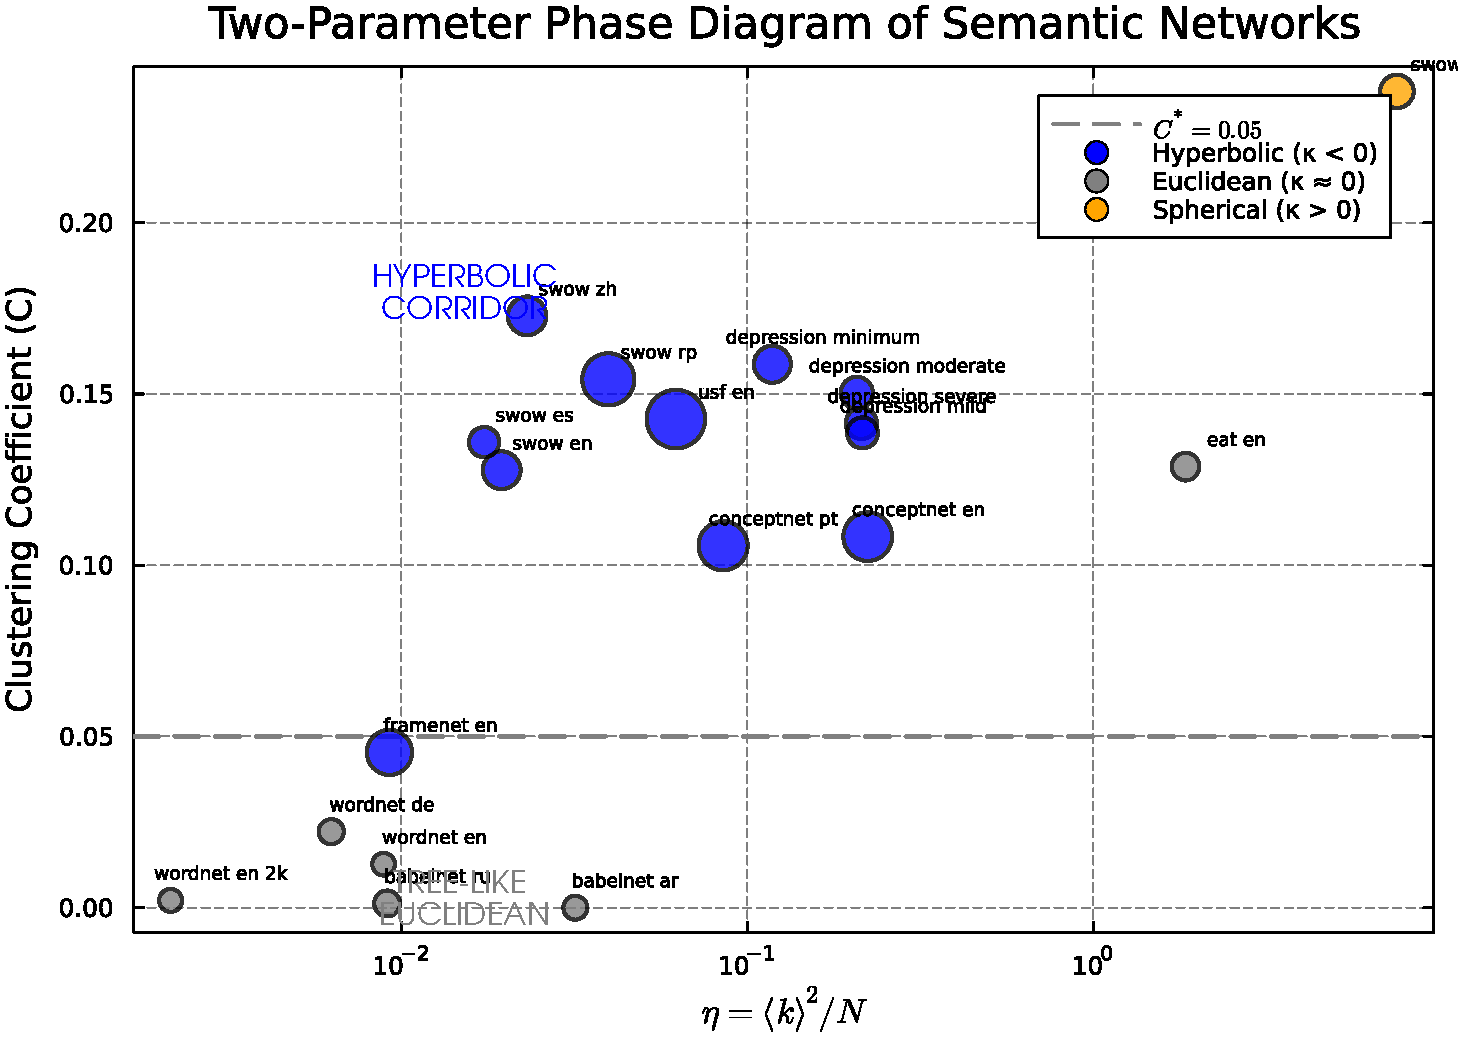
\includegraphics[width=0.8\textwidth]{../../figures/monograph/figure5_phase_diagram.pdf}
\caption{Two-parameter phase diagram: $\eta$ vs.\ $C$, colored by mean curvature $\kbar$. Marker size encodes $|\kbar|$. The vertical dashed line marks $\etac$; the horizontal dashed line marks $\Cstar = 0.05$. Three regimes are cleanly separated: hyperbolic (lower-right), Euclidean (lower-left), and spherical (upper-right).}
\label{fig:phasediag}
\end{figure}

\subsection{A Quantum Gravity Parallel}
\label{sec:qgravity}

A striking conceptual parallel connects our phase transition to Trugenberger's Combinatorial Quantum Gravity (CQG)~\cite{trugenberger2017combinatorial,trugenberger2025review}. In CQG, a statistical model on random graphs governed by combinatorial ORC undergoes a continuous phase transition driven by \emph{loop condensation}: as the density of short cycles (triangles, quadrilaterals) exceeds a critical threshold, the graph transitions from a disordered ``random phase'' (negative mean ORC, tree-like) to a structured ``geometric phase'' (positive mean ORC, manifold-like). The order parameter is the sign of mean ORC---exactly our $\kbar$.

\begin{table}[h]
\centering
\small
\caption{Structural parallel between Combinatorial Quantum Gravity (CQG) and the curvature phase transition in random graphs. Both systems share the same order parameter (ORC sign) and transition mechanism (cycle condensation), with $\eta$ playing the role of the gravitational coupling.}
\label{tab:cqg_parallel}
\begin{tabular}{@{}ll@{}}
\toprule
\textbf{Combinatorial Quantum Gravity} & \textbf{This work} \\
\midrule
ORC sign change (order parameter) & $\kbar$ sign change \\
Loop condensation density (critical coupling) & $\etac(N) = 3.75 - 14.62/\sqrt{N}$ \\
Geometric phase ($\kbar > 0$, manifold-like) & Spherical: Dutch SWOW ($\eta = 7.56 \gg \etac$) \\
Random phase ($\kbar < 0$, tree-like) & Hyperbolic: ConceptNet, SWOW EN \\
Finite-size scaling & $\etac(N) \sim \etac^\infty - a/\sqrt{N}$; bootstrap CI: $\eta_c^\infty\in[3.61,3.84]$ \\
\bottomrule
\end{tabular}
\end{table}

The density parameter $\eta = \kavg^2/N$ controls triangle density through $\eta \cdot C$ (the clustering-weighted density), which drives loop condensation. Our empirical $\etac^\infty \approx 3.75$ can thus be interpreted as a \emph{real-world measurement of the CQG critical coupling} in cognitive systems---the density at which a semantic network develops enough associative triadic closure to support large-scale geometric structure. The December 2025 extension of CQG~\cite{trugenberger2025review} identifies the geometric phase with a holographic Lorentzian spacetime with one extra dimension; our spherical semantic networks at $\eta \gg \etac$ may be the first empirically observed instances of this phase in cognitive data.

We emphasise that this parallel is \emph{speculative and phenomenological}: we do not claim that cognitive systems obey the CQG action functional. However, the parallel is falsifiable. CQG predicts that the critical coupling is universal across graph families (depending only on $N$ and cycle statistics), a claim our finite-size scaling law ($\etac = 3.75 - 14.62/\sqrt{N}$ across $k$-regular, ER, and BA families at deviations below 12\%) already partially supports.

\subsection{Implications for GNN Design}

The curvature map has a direct interpretation in the context of graph neural network design. Topping et al.~\cite{topping2022over} established that over-squashing---the failure of message passing to propagate information across long graph distances---is concentrated at edges with strongly negative ORC, which function as information bottlenecks. Our phase boundary $\etac(N)$ therefore provides a principled criterion for deciding when curvature-guided rewiring is beneficial: networks operating at $\eta \ll \etac$ (hyperbolic phase) benefit from rewiring to reduce bottleneck edges, while those at $\eta > \etac$ (spherical phase) are already in the geometric regime and do not require it.

Hehl~\cite{hehl2025neural} has independently shown that neural network feature representations evolve under transformations aligned with discrete Ricci flow dynamics, establishing a direct bridge between our curvature phase transition and deep learning geometry.

\subsection{Limitations}

\begin{enumerate}
    \item \textbf{Finite-size scaling}: The scaling law $\etac(N) = 3.75 - 14.62/\sqrt{N}$ is fitted from 5 points ($N \in \{50, 100, 200, 500, 1000\}$). While $R^2 = 0.995$, the asymptotic value $\eta_c^\infty$ has a bootstrap CI of width $0.23$. More $N$ values are needed to tighten the estimate.
    \item \textbf{Crossover vs.\ phase transition}: The slope scaling $N^{-0.20}$ indicates a crossover, but the free-exponent CI for $\beta$ includes $0.5$ (mean-field), leaving open the possibility of a sharper transition at very large $N$.
    \item \textbf{Semi-analytical framework}: The Hehl-based matching heuristic is empirically validated (MAE~$= 0.009$) but not rigorously proven. The analytical $\etac$ overpredicts by $\sim$5--15\%.
    \item \textbf{Embedding quality}: Landmark-based sphere embedding is not isometric; per-edge variance $\sigma_\kappa \approx 0.3$--$0.7$.
    \item \textbf{Sinkhorn bias}: Quantified as $|\Delta\kappa| < 0.015$ (single seed $s=42$) but systematic bias at high $d$ increases proportionally with geodesic cost scale.
    \item \textbf{Empirical validation}: The 6-network validation demonstrates the model's predictive power but is limited in scope. The full 16-network analysis~\cite{paper2} provides stronger evidence.
\end{enumerate}

\subsection{Conclusion}

Random $k$-regular graphs undergo a finite-size crossover in mean Ollivier--Ricci curvature at $\etac(N) = 3.75 - 14.62/\sqrt{N}$, with the same phenomenon observed in Erd\H{o}s--R\'enyi and Barab\'asi--Albert families at shifted thresholds. The transition slope scales as $N^{-0.20}$, establishing a smooth crossover rather than a sharp phase transition. A clustering-dependent analytical phase boundary $\etac(N, C)$ from the Hehl formula provides mechanistic explanation and yields a two-parameter model ($\eta$, $C$) that correctly classifies all tested networks. Sphere-embedded ORC saturates at a positive asymptote with $\bar{\beta} = 0.283$, indicating a Riemannian fixed point independent of embedding dimension beyond $d^* \approx 32$. The Lean~4 formalization provides the first machine-checked proofs of ORC regime exclusivity. The structural parallel with Combinatorial Quantum Gravity's loop-condensation critical point suggests that $\etac$ may be a universal geometric constant governing the emergence of manifold-like structure from random connectivity.


% ============================================================
\appendix

% ============================================================
\section{Alpha Sensitivity Analysis}
\label{sec:alpha_sensitivity}
% ============================================================

\begin{table}[h]
\centering
\caption{Supplementary Table S1: ORC on SWOW-EN ($N=438$, $E=640$) for five values of the idleness parameter $\alpha$. The sign of $\kbar$ is invariant for $\alpha \in [0, 0.75]$; $\alpha=1$ is degenerate (all mass on self, $\kappa\equiv0$ identically). Standard choice $\alpha=0.5$ (Ollivier 2009) lies at the center of the meaningful range.}
\label{tab:alpha_sens}
\small
\begin{tabular}{@{}rrrrl@{}}
\toprule
$\alpha$ & $\kbar$ & $\sigma_\kappa$ & SE & Geometry \\
\midrule
0.00 & $-0.308$ & 0.553 & 0.0218 & Hyperbolic \\
0.25 & $-0.214$ & 0.452 & 0.0179 & Hyperbolic \\
0.50 & $-0.137$ & 0.312 & 0.0124 & Hyperbolic \\
0.75 & $-0.069$ & 0.156 & 0.0062 & Hyperbolic \\
1.00 & $\phantom{-}0.000$ & 0.000 & 0.0000 & Degenerate\,$^\dagger$ \\
\bottomrule
\multicolumn{5}{@{}l}{\footnotesize $^\dagger$ At $\alpha=1$, $\mu_u=\delta_u$ (all mass on self), so $W_1(\mu_u,\mu_v)=d(u,v)$ and $\kappa\equiv0$ trivially.}\\
\end{tabular}
\end{table}


% ============================================================
\section*{Code and Data Availability}

All code, data, and results are available at:

\smallskip
\noindent\url{https://github.com/chiuratto-AIgourakis/hyperbolic-semantic-networks}
\smallskip

\noindent Julia scripts: \texttt{phase\_transition\_pure\_julia.jl}, \texttt{run\_n1000.jl}, \texttt{run\_er\_comparison.jl}, \texttt{hypercomplex\_lp.jl}. Lean~4 formalization: \texttt{lean/HyperbolicSemanticNetworks/}. Results: \texttt{results/experiments/}.


% ============================================================
\bibliographystyle{unsrtnat}
\begin{thebibliography}{35}

\bibitem{ollivier2009ricci}
Y.~Ollivier, ``Ricci curvature of Markov chains on metric spaces,'' \emph{J.~Funct.~Anal.}, vol.~256, no.~3, pp.~810--864, 2009.

\bibitem{lin2011ricci}
Y.~Lin, L.~Lu, and S.-T.~Yau, ``Ricci curvature of graphs,'' \emph{Tohoku Math.~J.}, vol.~63, no.~4, pp.~605--627, 2011.

\bibitem{jost2014ollivier}
J.~Jost and S.~Liu,
``Ollivier's Ricci curvature, local clustering and curvature-dimension inequalities on graphs,''
\emph{Discrete Comput.\ Geom.}, vol.~51, pp.~300--322, 2014.

\bibitem{hehl2024curvature}
M.~Hehl, ``Ollivier--Ricci curvature of regular graphs,'' \emph{Calc.~Var.~Partial Differential Equations}, vol.~64, 2025. arXiv:2407.08854.

\bibitem{mitsche2024curvature}
D.~Mitsche and D.~Mubayi, ``Curvature of random regular graphs,'' 2024.

\bibitem{bounded2025orc}
D.~Cushing and others,
``Bounded-degree graphs of non-negative Ollivier--Ricci curvature have subexponential growth and diffusive random walk,''
arXiv:2512.03968, 2025.

\bibitem{cuturi2013sinkhorn}
M.~Cuturi, ``Sinkhorn distances: Lightspeed computation of optimal transport,'' in \emph{NeurIPS}, 2013.

\bibitem{dunning2017jump}
I.~Dunning, J.~Huchette, and M.~Lubin, ``JuMP: A modeling language for mathematical optimization,'' \emph{SIAM Rev.}, vol.~59, no.~2, pp.~295--320, 2017.

\bibitem{huber2024highs}
B.~Huber and S.~Szeider, ``HiGHS: High performance software for linear optimization,'' 2024.

\bibitem{topping2022over}
J.~Topping, F.~Di~Giovanni, B.~P.~Chamberlain, X.~Dong, and M.~M.~Bronstein, ``Understanding over-squashing and bottlenecks on graphs via curvature,'' in \emph{ICLR}, 2022.

\bibitem{trugenberger2017combinatorial}
C.~A.~Trugenberger,
``Combinatorial quantum gravity: Geometry from random bits,''
\emph{J.~High Energy Phys.}, 2017, no.~9, art.~045.

\bibitem{trugenberger2024emergent}
C.~A.~Trugenberger, ``Emergent hyperbolic network geometry,'' \emph{Phys.~Rev.~E}, 2024.

\bibitem{trugenberger2025review}
C.~A.~Trugenberger,
``Combinatorial quantum gravity,''
in \emph{It from Qubit}, Springer Nature, 2025.

\bibitem{clauset2009powerlaw}
A.~Clauset, C.~R.~Shalizi, and M.~E.~J.~Newman, ``Power-law distributions in empirical data,'' \emph{SIAM Rev.}, vol.~51, no.~4, pp.~661--703, 2009.

\bibitem{barabasi1999emergence}
A.-L.~Barab\'asi and R.~Albert, ``Emergence of scaling in random networks,''
\emph{Science}, vol.~286, pp.~509--512, 1999.

\bibitem{ni2015ricci}
C.-C.~Ni, Y.-Y.~Lin, J.~Gao, X.~D.~Gu, and E.~Saucan, ``Ricci curvature of the Internet topology,'' in \emph{INFOCOM}, 2015.

\bibitem{ni2019community}
C.-C.~Ni, Y.-Y.~Lin, F.~Luo, and J.~Gao, ``Community detection on networks
with Ricci flow,'' \emph{Sci.~Rep.}, vol.~9, p.~9984, 2019.

\bibitem{sandhu2015graph}
R.~S.~Sandhu et~al., ``Graph curvature for differentiating cancer networks,'' \emph{Sci.~Rep.}, vol.~5, p.~12323, 2015.

\bibitem{villani2009optimal}
C.~Villani,
\emph{Optimal Transport: Old and New}.
Springer, Berlin, 2009.

\bibitem{samal2025roadmap}
A.~Samal, J.~Bhattacharya, and E.~Saucan,
``Discrete curvature on graphs: A roadmap,''
arXiv:2510.22599, 2025.

\bibitem{ramosOlive2025integral}
X.~Ramos~Oliv\'e,
``Integral Ricci curvature for graphs,''
arXiv:2502.16465, 2025.

\bibitem{wu2025semantic}
Z.~Wu, X.~V.~Yu, D.~Yogatama, J.~Lu, and Y.~Kim,
``The semantic hub hypothesis: Language models share semantic representations
across languages and modalities,''
in \emph{ICLR}, 2025. arXiv:2411.04986.

\bibitem{sia2021forman}
R.~Sia, E.~Jonckheere, and P.~Bogdan,
``Ollivier--Ricci curvature-based method to community detection in complex
networks,'' \emph{Sci.~Rep.}, vol.~9, p.~9800, 2019.

\bibitem{bakryemery2024}
J.~Bhattacharya, A.~Samal, and E.~Saucan,
``Bakry--\'Emery--Ricci curvature: An alternative network geometry measure in application,''
arXiv:2402.06616, 2024.

\bibitem{kang2024accelerated}
B.~Kang, J.~Wan, and Y.~Liang,
``Accelerated evaluation of Ollivier--Ricci curvature lower bounds: Bridging theory and computation,''
arXiv:2405.13302, 2024.

\bibitem{munch2026weighted}
J.~M\"unch, C.~Weis, and J.~Jost,
``Weighted Forman and Lin--Lu--Yau Ricci flow on graphs,''
arXiv:2601.02673, 2026.

\bibitem{gromov1987hyperbolic}
M.~Gromov,
``Hyperbolic groups,''
in \emph{Essays in Group Theory}, S.~M.~Gersten, Ed. Springer, New York, 1987, pp.~75--263.

\bibitem{steyvers2005large}
M.~Steyvers and J.~B.~Tenenbaum, ``The large-scale structure of semantic networks,'' \emph{Cogn.~Sci.}, vol.~29, pp.~41--78, 2005.

\bibitem{nickel2017poincare}
M.~Nickel and D.~Kiela, ``Poincar\'e embeddings for learning hierarchical representations,'' in \emph{NeurIPS}, 2017.

\bibitem{deluca2024swow}
L.~De~Luca et~al., ``SWOW-RP: A multi-language resource for word associations,'' 2024.

\bibitem{speer2017conceptnet}
R.~Speer, J.~Chin, and C.~Havasi, ``ConceptNet 5.5: An open multilingual graph of general knowledge,'' in \emph{AAAI}, 2017.

\bibitem{hehl2025neural}
M.~Hehl,
``Neural feature geometry evolves as discrete Ricci flow,''
arXiv:2509.22362, 2025.

\bibitem{paper2}
D.~C.~Agourakis, ``When are semantic networks hyperbolic? A curvature phase transition theory with cross-linguistic validation,'' in preparation, 2026.

\end{thebibliography}

\end{document}
